% !TEX TS-program = pdflatex
\documentclass[11pt]{article}

% -------------------- Packages --------------------
\usepackage[a4paper,margin=1in]{geometry}
\usepackage{amsmath,amssymb}
\usepackage[T1]{fontenc}
\usepackage{lmodern}
\usepackage{xcolor}
\usepackage{tcolorbox}
\tcbuselibrary{skins,breakable}
\usepackage{enumitem}
\usepackage{hyperref}
\usepackage{tikz}
\usetikzlibrary{calc,angles,quotes,arrows.meta,intersections}

\pagestyle{empty}

% -------------------- Dark Theme Colors --------------------
\definecolor{bg}{HTML}{000000}
\definecolor{pairbg}{HTML}{121212}
\definecolor{solbg}{HTML}{0A0A0A}
\definecolor{border}{HTML}{2A2A2A}
\definecolor{text}{HTML}{FFFFFF}
\definecolor{muted}{HTML}{C9CDD3}
\definecolor{gold}{HTML}{FFD700}
\definecolor{green}{HTML}{4ADE80}
\definecolor{cyan}{HTML}{38BDF8}

\pagecolor{bg}
\color{text}

\hypersetup{
  colorlinks=true,
  linkcolor=cyan,
  urlcolor=cyan
}

\setlength{\parindent}{0pt}
\setlength{\parskip}{10pt}

% Help LaTeX avoid overfull lines globally
\sloppy
\setlength{\emergencystretch}{3em}

\setlist[itemize]{left=1.4em,itemsep=6pt,topsep=6pt}
\setlist[enumerate]{left=1.6em,itemsep=4pt,topsep=4pt}

% -------------------- tcolorbox Base --------------------
\tcbset{
  enhanced,
  breakable,
  arc=12pt,
  boxrule=0.8pt,
  left=14pt,right=14pt,top=12pt,bottom=12pt
}

\newtcolorbox{QAPair}[1]{%
  colback=pairbg,
  colbacklower=solbg,
  colframe=border,
  coltext=text,
  title=\textcolor{gold}{\bfseries #1},
  fonttitle=\bfseries,
  coltitle=text,
  segmentation style={draw=border, dashed, line width=0.6pt},
  before upper=\raggedright,
  before lower=\raggedright
}

\newtcolorbox{QuickBox}{%
  colback=pairbg,
  colframe=cyan,
  coltext=text,
  fontupper=\color{text}\raggedright,
  borderline north={4pt}{0pt}{cyan},
  arc=14pt,
  boxrule=0.8pt
}

% Helper for step headings
\newcommand{\Step}[1]{\textcolor{muted}{\textbf{Step #1:}}}

% Small centered diagram block (for step-by-step visuals)
\newenvironment{StepDiagram}{\par\medskip\begin{center}}{\end{center}\medskip}

% TikZ styles
\tikzset{
  base/.style={draw=text, line width=0.9pt, line cap=round, line join=round},
  new/.style={draw=cyan, line width=1.2pt, line cap=round, line join=round},
  help/.style={draw=muted, dashed, line width=0.9pt},
  ang/.style={draw=gold, line width=1.0pt},
  dot/.style={circle, fill=text, inner sep=1.2pt},
  lab/.style={text=text, font=\small},
  labm/.style={text=muted, font=\small},
}

% -------------------- IMPORTANT FIX --------------------
% EqDiagram is MATH-MODE SAFE: write math inside without $...$
\newcommand{\EqDiagram}[1]{%
\begin{StepDiagram}
\begin{tikzpicture}
\node[
  draw=border,
  rounded corners=10pt,
  inner sep=8pt,
  text=text,
  align=left,
  text width=0.85\linewidth
] {\(\displaystyle #1\)};
\end{tikzpicture}
\end{StepDiagram}
}

% ============================================================
\begin{document}

\begin{center}
{\LARGE\bfseries \textcolor{gold}{Exercise 10.2 --- Solutions}}\\[-2pt]
\end{center}

% -------------------- Quick formulas + diagram PER LINE --------------------
\begin{QuickBox}
{\color{cyan}\bfseries Quick formulas (Angles \& tangents in a circle)}\par\medskip

\begin{itemize}
\item \textbf{Angle at centre is double the angle at circumference (same arc):}
\[
\angle AOB = 2\,\angle ACB.
\]
\begin{StepDiagram}
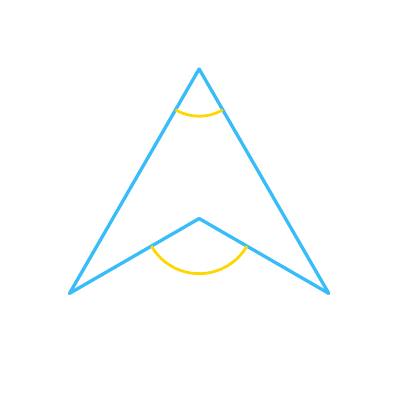
\begin{tikzpicture}[scale=0.95]
  \def\r{2.0}
  \coordinate (O) at (0,0);
  \coordinate (A) at ({\r*cos(210)},{\r*sin(210)});
  \coordinate (B) at ({\r*cos(330)},{\r*sin(330)});
  \coordinate (C) at ({\r*cos(90)},{\r*sin(90)});
  \draw[base] (O) circle (\r);
  \node[dot,label={[lab]below:$O$}] at (O) {};
  \node[dot,label={[lab]below left:$A$}] at (A) {};
  \node[dot,label={[lab]below right:$B$}] at (B) {};
  \node[dot,label={[lab]above:$C$}] at (C) {};
  \draw[new] (O)--(A) (O)--(B);
  \draw[new] (C)--(A) (C)--(B);
  \pic[ang,"$2x$",lab,angle radius=7mm,angle eccentricity=1.2] {angle=A--O--B};
  \pic[ang,"$x$",lab,angle radius=6mm,angle eccentricity=1.2] {angle=A--C--B};
\end{tikzpicture}
\end{StepDiagram}

\item \textbf{Angles in the same segment are equal (same chord):}
\[
\angle APB=\angle AQB.
\]
\begin{StepDiagram}
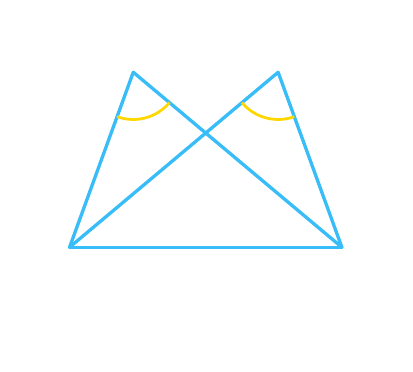
\begin{tikzpicture}[scale=0.92]
  \def\r{2.0}
  \coordinate (O) at (0,0);
  \coordinate (A) at ({\r*cos(200)},{\r*sin(200)});
  \coordinate (B) at ({\r*cos(340)},{\r*sin(340)});
  \coordinate (P) at ({\r*cos(120)},{\r*sin(120)});
  \coordinate (Q) at ({\r*cos(60)},{\r*sin(60)});
  \draw[base] (O) circle (\r);
  \foreach \X/\pos in {A/below left,B/below right,P/above left,Q/above right}
    \node[dot,label={[lab]\pos:$\X$}] at (\X) {};
  \draw[new] (A)--(B);
  \draw[new] (P)--(A) (P)--(B);
  \draw[new] (Q)--(A) (Q)--(B);
  \pic[ang,"$x$",lab,angle radius=6mm,angle eccentricity=1.2] {angle=A--P--B};
  \pic[ang,"$x$",lab,angle radius=6mm,angle eccentricity=1.2] {angle=A--Q--B};
\end{tikzpicture}
\end{StepDiagram}

\item \textbf{Angle in a semicircle is a right angle:}
\[
AB\text{ is diameter } \Rightarrow \angle ACB=90^\circ.
\]
\begin{StepDiagram}
\begin{tikzpicture}[scale=0.92]
  \def\r{2.0}
  \coordinate (O) at (0,0);
  \coordinate (A) at (-\r,0);
  \coordinate (B) at (\r,0);
  \coordinate (C) at ({\r*cos(70)},{\r*sin(70)});
  \draw[base] (O) circle (\r);
  \node[dot,label={[lab]below:$O$}] at (O) {};
  \node[dot,label={[lab]left:$A$}] at (A) {};
  \node[dot,label={[lab]right:$B$}] at (B) {};
  \node[dot,label={[lab]above:$C$}] at (C) {};
  \draw[new] (A)--(B) (A)--(C) (C)--(B);
  \draw[base] ($(C)+(-0.18,0)$) -- ($(C)+(-0.18,-0.18)$) -- ($(C)+(0,-0.18)$);
\end{tikzpicture}
\end{StepDiagram}

\item \textbf{Tangent--chord theorem:} angle between tangent and chord equals the angle in the opposite segment.
\begin{StepDiagram}
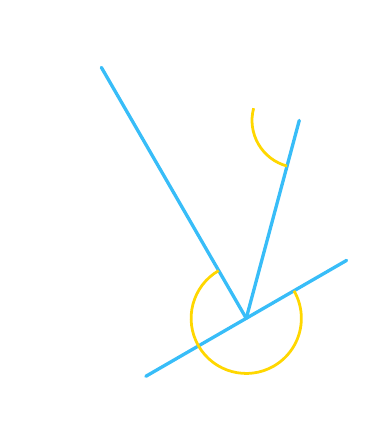
\begin{tikzpicture}[scale=0.92]
  \def\r{2.0}
  \coordinate (O) at (0,0);
  \coordinate (B) at ({\r*cos(300)},{\r*sin(300)});
  \coordinate (A) at ({\r*cos(120)},{\r*sin(120)});
  \coordinate (C) at ({\r*cos(30)},{\r*sin(30)});
  % tangent at B: direction perpendicular to OB
  \coordinate (T1) at ($(B)+({-1.6*sin(300)},{1.6*cos(300)})$);
  \coordinate (T2) at ($(B)+({ 1.6*sin(300)},{-1.6*cos(300)})$);
  \draw[base] (O) circle (\r);
  \node[dot,label={[lab]below:$O$}] at (O) {};
  \node[dot,label={[lab]below right:$B$}] at (B) {};
  \node[dot,label={[lab]above left:$A$}] at (A) {};
  \node[dot,label={[lab]above right:$C$}] at (C) {};
  \draw[new] (B)--(A);
  \draw[new] (B)--(C);
  \draw[new] (T1)--(T2);
  \pic[ang,"$x$",lab,angle radius=7mm,angle eccentricity=1.2] {angle=A--B--T1};
  \pic[ang,"$x$",lab,angle radius=6mm,angle eccentricity=1.2] {angle=A--C--B};
\end{tikzpicture}
\end{StepDiagram}

\end{itemize}
\end{QuickBox}

% ============================================================
% Q1
\begin{QAPair}{Question 1}
\textcolor{gold}{\bfseries Question:} In the adjoining figure, $\angle P=30^\circ$.
Find the values of $\angle Q$ and $\angle ROS$.
\tcblower
\textcolor{green}{\bfseries Answer:}\par

\Step{1} $\angle P$ subtends chord $RS$. Angles in the same segment are equal, so $\angle Q=\angle P=30^\circ$.

\begin{StepDiagram}
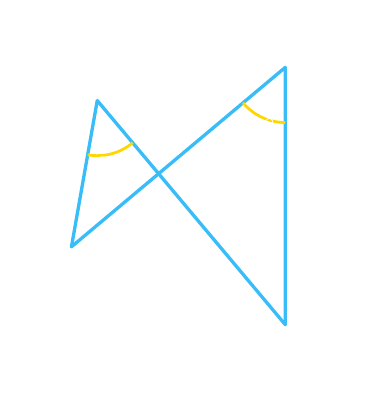
\begin{tikzpicture}[scale=0.92]
  \def\r{2.05}
  \coordinate (O) at (0,0);
  \coordinate (R) at ({\r*cos(200)},{\r*sin(200)});
  \coordinate (S) at ({\r*cos(300)},{\r*sin(300)});
  \coordinate (P) at ({\r*cos(60)},{\r*sin(60)});
  \coordinate (Q) at ({\r*cos(140)},{\r*sin(140)});
  \draw[base] (O) circle (\r);
  \node[dot,label={[lab]below:$O$}] at (O) {};
  \foreach \X/\pos in {R/left,S/below right,P/above right,Q/above left}
    \node[dot,label={[lab]\pos:$\X$}] at (\X) {};
  \draw[new] (P)--(R) (P)--(S);
  \draw[new] (Q)--(R) (Q)--(S);
  \pic[ang,"$30^\circ$",lab,angle radius=7mm,angle eccentricity=1.2] {angle=R--P--S};
  \pic[ang,"$30^\circ$",lab,angle radius=7mm,angle eccentricity=1.2] {angle=R--Q--S};
\end{tikzpicture}
\end{StepDiagram}

\Step{2} The angle at the centre on the same chord $RS$ is double:
\[
\angle ROS = 2\angle RPS = 60^\circ.
\]

\begin{StepDiagram}
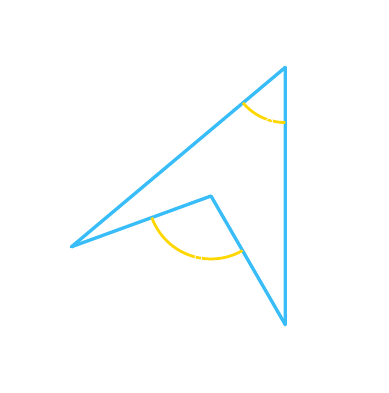
\begin{tikzpicture}[scale=0.92]
  \def\r{2.05}
  \coordinate (O) at (0,0);
  \coordinate (R) at ({\r*cos(200)},{\r*sin(200)});
  \coordinate (S) at ({\r*cos(300)},{\r*sin(300)});
  \coordinate (P) at ({\r*cos(60)},{\r*sin(60)});
  \draw[base] (O) circle (\r);
  \foreach \X/\pos in {O/below,R/left,S/below right,P/above right}
    \node[dot,label={[lab]\pos:$\X$}] at (\X) {};
  \draw[new] (O)--(R) (O)--(S);
  \draw[new] (P)--(R) (P)--(S);
  \pic[ang,"$60^\circ$",lab,angle radius=8mm,angle eccentricity=1.15] {angle=R--O--S};
  \pic[ang,"$30^\circ$",lab,angle radius=7mm,angle eccentricity=1.2] {angle=R--P--S};
\end{tikzpicture}
\end{StepDiagram}

\EqDiagram{\angle Q=30^\circ,\qquad \angle ROS=60^\circ.}

\[
\boxed{\angle Q=30^\circ \qquad \angle ROS=60^\circ}
\]
\end{QAPair}

% ============================================================
% Q2
\begin{QAPair}{Question 2}
\textcolor{gold}{\bfseries Question:} In the adjoining figure, $\angle BAO=30^\circ$.
Find $\angle ABO$, $\angle AOB$, $\angle ACB$.
\tcblower
\textcolor{green}{\bfseries Answer:}\par

\Step{1} $OA=OB$ (radii) so $\triangle AOB$ is isosceles and
\[
\angle ABO=\angle BAO=30^\circ.
\]

\begin{StepDiagram}
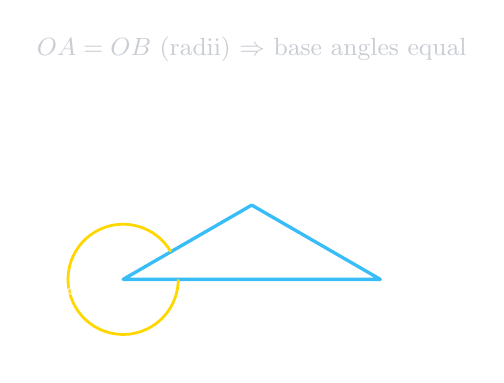
\begin{tikzpicture}[scale=0.92]
  \def\r{2.05}
  \coordinate (O) at (0,0);
  \coordinate (A) at ({\r*cos(210)},{\r*sin(210)});
  \coordinate (B) at ({\r*cos(330)},{\r*sin(330)});
  \draw[base] (O) circle (\r);
  \foreach \X/\pos in {O/below,A/below left,B/below right}
    \node[dot,label={[lab]\pos:$\X$}] at (\X) {};
  \draw[new] (O)--(A) (O)--(B) (A)--(B);
  \node[labm] at (0,2.15) {$OA=OB$ (radii) $\Rightarrow$ base angles equal};
  \pic[ang,"$30^\circ$",lab,angle radius=7mm,angle eccentricity=1.2] {angle=O--A--B};
\end{tikzpicture}
\end{StepDiagram}

\Step{2} Sum of angles in $\triangle AOB$:
\[
\angle AOB = 180^\circ - 30^\circ - 30^\circ = 120^\circ.
\]

\begin{StepDiagram}
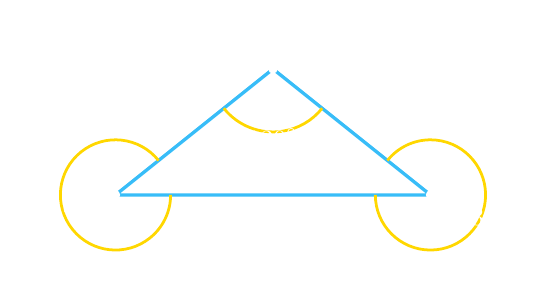
\begin{tikzpicture}[scale=1.0]
  \coordinate (A) at (-2,0);
  \coordinate (B) at (2,0);
  \coordinate (O) at (0,1.6);
  \draw[new] (A)--(O)--(B)--cycle;
  \foreach \X/\pos in {A/below,B/below,O/above}
    \node[dot,label={[lab]\pos:$\X$}] at (\X) {};
  \pic[ang,"$30^\circ$",lab,angle radius=7mm,angle eccentricity=1.15] {angle=O--A--B};
  \pic[ang,"$30^\circ$",lab,angle radius=7mm,angle eccentricity=1.15] {angle=A--B--O};
  \pic[ang,"$120^\circ$",lab,angle radius=8mm,angle eccentricity=1.10] {angle=A--O--B};
\end{tikzpicture}
\end{StepDiagram}

\Step{3} Angle at circumference subtending chord $AB$ is half the central angle:
\[
\angle ACB=\frac12\,\angle AOB=\frac12(120^\circ)=60^\circ.
\]

\begin{StepDiagram}
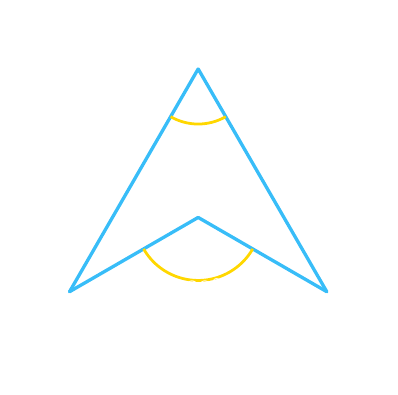
\begin{tikzpicture}[scale=0.92]
  \def\r{2.05}
  \coordinate (O) at (0,0);
  \coordinate (A) at ({\r*cos(210)},{\r*sin(210)});
  \coordinate (B) at ({\r*cos(330)},{\r*sin(330)});
  \coordinate (C) at ({\r*cos(90)},{\r*sin(90)});
  \draw[base] (O) circle (\r);
  \foreach \X/\pos in {O/below,A/below left,B/below right,C/above}
    \node[dot,label={[lab]\pos:$\X$}] at (\X) {};
  \draw[new] (O)--(A) (O)--(B);
  \draw[new] (C)--(A) (C)--(B);
  \pic[ang,"$120^\circ$",lab,angle radius=8mm,angle eccentricity=1.12] {angle=A--O--B};
  \pic[ang,"$60^\circ$",lab,angle radius=7mm,angle eccentricity=1.2] {angle=A--C--B};
\end{tikzpicture}
\end{StepDiagram}

\[
\boxed{\angle ABO=30^\circ,\quad \angle AOB=120^\circ,\quad \angle ACB=60^\circ}
\]
\end{QAPair}

% ============================================================
% Q3
\begin{QAPair}{Question 3}
\textcolor{gold}{\bfseries Question:} In the adjoining figure, $\angle BAC=40^\circ$ and $\angle ACD=60^\circ$.
Find $\angle ABC$, $\angle BCA$, $\angle CAD$.
\tcblower
\textcolor{green}{\bfseries Answer:}\par

\Step{1} $AC$ is a diameter $\Rightarrow$ angle in a semicircle:
\[
\angle ABC=90^\circ.
\]

\begin{StepDiagram}
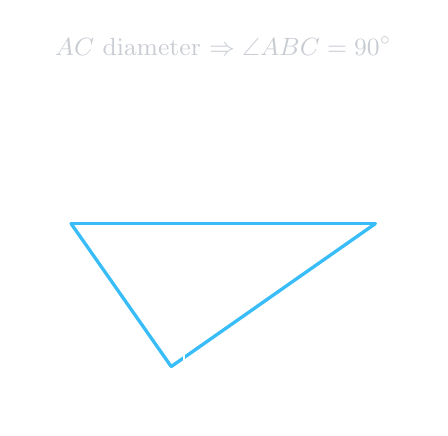
\begin{tikzpicture}[scale=0.92]
  \def\r{2.1}
  \coordinate (O) at (0,0);
  \coordinate (A) at (-\r,0);
  \coordinate (C) at (\r,0);
  \coordinate (B) at ({\r*cos(250)},{\r*sin(250)});
  \draw[base] (O) circle (\r);
  \foreach \X/\pos in {A/left,C/right,B/below}
    \node[dot,label={[lab]\pos:$\X$}] at (\X) {};
  \draw[new] (A)--(C); % diameter
  \draw[new] (A)--(B) (B)--(C);
  \draw[base] ($(B)+(0.18,0)$) -- ($(B)+(0.18,0.18)$) -- ($(B)+(0,0.18)$);
  \node[labm] at (0,2.45) {$AC$ diameter $\Rightarrow \angle ABC=90^\circ$};
\end{tikzpicture}
\end{StepDiagram}

\Step{2} In $\triangle ABC$:
\[
\angle BCA = 180^\circ - 90^\circ - 40^\circ = 50^\circ.
\]

\begin{StepDiagram}
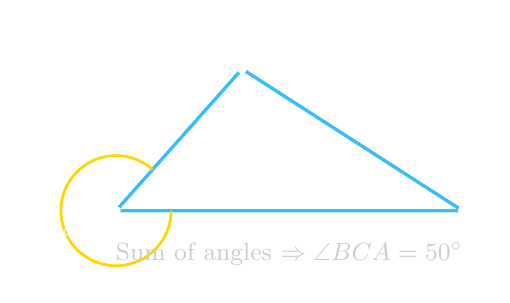
\begin{tikzpicture}[scale=1.0]
  \coordinate (A) at (-2.2,0);
  \coordinate (C) at (2.2,0);
  \coordinate (B) at (-0.6,1.8);
  \draw[new] (A)--(B)--(C)--cycle;
  \foreach \X/\pos in {A/below,C/below,B/above}
    \node[dot,label={[lab]\pos:$\X$}] at (\X) {};
  \draw[base] ($(B)+(0.18,0)$) -- ($(B)+(0.18,0.18)$) -- ($(B)+(0,0.18)$);
  \pic[ang,"$40^\circ$",lab,angle radius=7mm,angle eccentricity=1.2] {angle=B--A--C};
  \node[labm] at (0,-0.55) {Sum of angles $\Rightarrow \angle BCA=50^\circ$};
\end{tikzpicture}
\end{StepDiagram}

\Step{3} In $\triangle ACD$, $AC$ is diameter $\Rightarrow \angle ADC=90^\circ$.
So
\[
\angle CAD = 180^\circ - 90^\circ - 60^\circ = 30^\circ.
\]

\begin{StepDiagram}
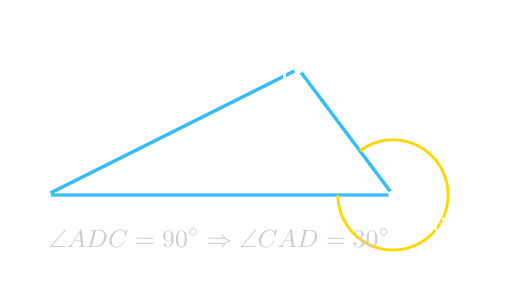
\begin{tikzpicture}[scale=1.0]
  \coordinate (A) at (-2.2,0);
  \coordinate (C) at (2.2,0);
  \coordinate (D) at (1.0,1.6);
  \draw[new] (A)--(D)--(C)--cycle;
  \foreach \X/\pos in {A/below,C/below,D/above}
    \node[dot,label={[lab]\pos:$\X$}] at (\X) {};
  \draw[base] ($(D)+(-0.18,0)$) -- ($(D)+(-0.18,-0.18)$) -- ($(D)+(0,-0.18)$);
  \pic[ang,"$60^\circ$",lab,angle radius=7mm,angle eccentricity=1.2] {angle=A--C--D};
  \node[labm] at (0,-0.55) {$\angle ADC=90^\circ \Rightarrow \angle CAD=30^\circ$};
\end{tikzpicture}
\end{StepDiagram}

\[
\boxed{\angle ABC=90^\circ,\quad \angle BCA=50^\circ,\quad \angle CAD=30^\circ}
\]
\end{QAPair}

% ============================================================
% Q4
\begin{QAPair}{Question 4}
\textcolor{gold}{\bfseries Question:} In the figure, $AOB$ is an equilateral triangle.
Find the measures of $\angle O$ and $\angle C$.
\tcblower
\textcolor{green}{\bfseries Answer:}\par

\Step{1} Equilateral $\triangle AOB$ $\Rightarrow$
\[
\angle AOB = 60^\circ.
\]

\begin{StepDiagram}
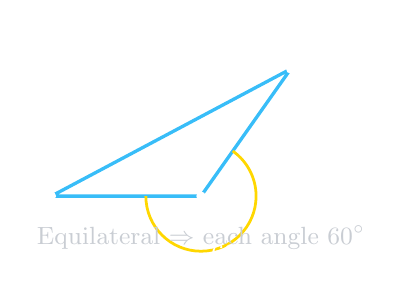
\begin{tikzpicture}[scale=0.95]
  \coordinate (O) at (0,0);
  \coordinate (A) at (-2,0);
  \coordinate (B) at (1.2,1.7);
  \draw[new] (O)--(A)--(B)--cycle;
  \foreach \X/\pos in {O/below,A/below,B/above}
    \node[dot,label={[lab]\pos:$\X$}] at (\X) {};
  \pic[ang,"$60^\circ$",lab,angle radius=7mm,angle eccentricity=1.15] {angle=A--O--B};
  \node[labm] at (0,-0.55) {Equilateral $\Rightarrow$ each angle $60^\circ$};
\end{tikzpicture}
\end{StepDiagram}

\Step{2} $\angle C$ subtends chord $AB$, so it is half the central angle:
\[
\angle C = \frac12\,\angle AOB = 30^\circ.
\]

\begin{StepDiagram}
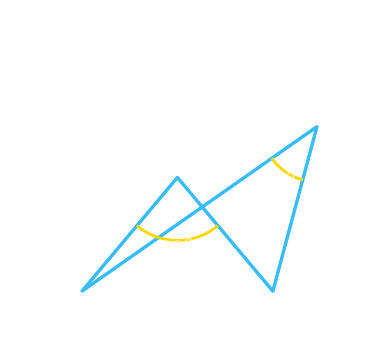
\begin{tikzpicture}[scale=0.92]
  \def\r{2.05}
  \coordinate (O) at (0,0);
  \coordinate (A) at ({\r*cos(230)},{\r*sin(230)});
  \coordinate (B) at ({\r*cos(310)},{\r*sin(310)});
  \coordinate (C) at ({\r*cos(20)},{\r*sin(20)});
  \draw[base] (O) circle (\r);
  \foreach \X/\pos in {O/below,A/below left,B/below right,C/right}
    \node[dot,label={[lab]\pos:$\X$}] at (\X) {};
  \draw[new] (O)--(A) (O)--(B);
  \draw[new] (C)--(A) (C)--(B);
  \pic[ang,"$60^\circ$",lab,angle radius=8mm,angle eccentricity=1.12] {angle=A--O--B};
  \pic[ang,"$30^\circ$",lab,angle radius=7mm,angle eccentricity=1.2] {angle=A--C--B};
\end{tikzpicture}
\end{StepDiagram}

\[
\boxed{\angle O=60^\circ \qquad \angle C=30^\circ}
\]
\end{QAPair}

% ============================================================
% Q5
\begin{QAPair}{Question 5}
\textcolor{gold}{\bfseries Question:} In the figure, $AB\parallel CD$.
Find the values of $\angle AEB$, $\angle B$, $\angle C$ and $\angle D$.
\tcblower
\textcolor{green}{\bfseries Answer:}\par

\Step{1} Vertical opposite angles are equal:
\[
\angle AEB = \angle CED = 110^\circ.
\]

\begin{StepDiagram}
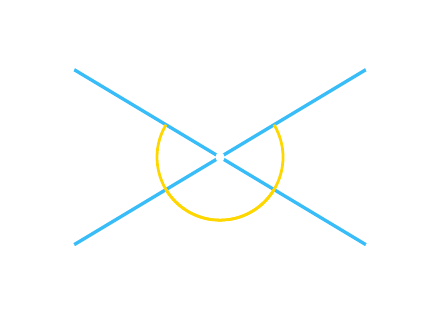
\begin{tikzpicture}[scale=0.95]
  \coordinate (E) at (0,0);
  \coordinate (A) at (-2,-1.2);
  \coordinate (D) at (2,1.2);
  \coordinate (B) at (2,-1.2);
  \coordinate (C) at (-2,1.2);
  \draw[new] (A)--(D);
  \draw[new] (B)--(C);
  \node[dot,label={[lab]below left:$A$}] at (A) {};
  \node[dot,label={[lab]below right:$B$}] at (B) {};
  \node[dot,label={[lab]above left:$C$}] at (C) {};
  \node[dot,label={[lab]above right:$D$}] at (D) {};
  \node[dot,label={[lab]right:$E$}] at (E) {};
  \pic[ang,"$110^\circ$",lab,angle radius=8mm,angle eccentricity=1.15] {angle=C--E--D};
  \pic[ang,"$110^\circ$",lab,angle radius=8mm,angle eccentricity=1.15] {angle=A--E--B};
\end{tikzpicture}
\end{StepDiagram}

\Step{2} In $\triangle AEB$ (with $\angle EAB=30^\circ$):
\[
\angle B = 180^\circ - 110^\circ - 30^\circ = 40^\circ.
\]

\begin{StepDiagram}
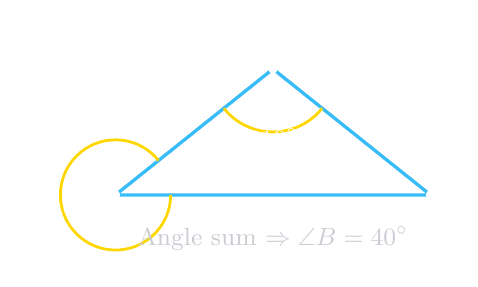
\begin{tikzpicture}[scale=1.0]
  \coordinate (A) at (-2,0);
  \coordinate (B) at (2,0);
  \coordinate (E) at (0,1.6);
  \draw[new] (A)--(E)--(B)--cycle;
  \foreach \X/\pos in {A/below,B/below,E/above}
    \node[dot,label={[lab]\pos:$\X$}] at (\X) {};
  \pic[ang,"$30^\circ$",lab,angle radius=7mm,angle eccentricity=1.15] {angle=E--A--B};
  \pic[ang,"$110^\circ$",lab,angle radius=8mm,angle eccentricity=1.10] {angle=A--E--B};
  \node[labm] at (0,-0.55) {Angle sum $\Rightarrow \angle B=40^\circ$};
\end{tikzpicture}
\end{StepDiagram}

\Step{3} Since $AB\parallel CD$, alternate interior angles give:
\[
\angle C = \angle B = 40^\circ.
\]

\begin{StepDiagram}
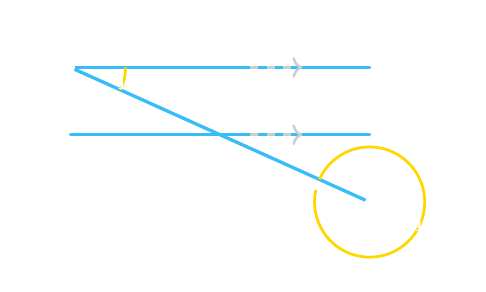
\begin{tikzpicture}[scale=0.95]
  \coordinate (B) at (2,0);
  \coordinate (C) at (-2,1.8);
  \coordinate (A1) at (-2,0.9);
  \coordinate (B1) at (2,0.9);
  \coordinate (C1) at (-2,1.8);
  \coordinate (D1) at (2,1.8);
  \draw[new] (A1)--(B1);
  \draw[new] (C1)--(D1);
  \draw[new] (B)--(C);
  \node[dot,label={[lab]below:$B$}] at (B) {};
  \node[dot,label={[lab]above left:$C$}] at (C) {};
  \draw[help,->] ($(A1)!0.6!(B1)$) -- ($(A1)!0.6!(B1)+(0.7,0)$);
  \draw[help,->] ($(C1)!0.6!(D1)$) -- ($(C1)!0.6!(D1)+(0.7,0)$);
  \pic[ang,"$40^\circ$",lab,angle radius=7mm,angle eccentricity=1.15] {angle=A1--B--C};
  \pic[ang,"$40^\circ$",lab,angle radius=7mm,angle eccentricity=1.15] {angle=B--C--D1};
\end{tikzpicture}
\end{StepDiagram}

\Step{4} Since $AB\parallel CD$, corresponding angles give:
\[
\angle D = \angle DAB = 30^\circ.
\]

\begin{StepDiagram}
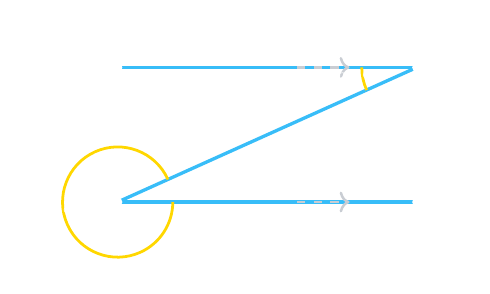
\begin{tikzpicture}[scale=0.95]
  \coordinate (A) at (-2,0);
  \coordinate (B) at (2,0);
  \coordinate (C) at (-2,1.8);
  \coordinate (D) at (2,1.8);
  \coordinate (Aup) at (-2,0);
  \coordinate (Dup) at (2,1.8);
  \draw[new] (A)--(B);
  \draw[new] (C)--(D);
  \draw[new] (A)--(D);
  \draw[help,->] ($(A)!0.6!(B)$) -- ($(A)!0.6!(B)+(0.7,0)$);
  \draw[help,->] ($(C)!0.6!(D)$) -- ($(C)!0.6!(D)+(0.7,0)$);
  \node[dot,label={[lab]below left:$A$}] at (A) {};
  \node[dot,label={[lab]below right:$B$}] at (B) {};
  \node[dot,label={[lab]above left:$C$}] at (C) {};
  \node[dot,label={[lab]above right:$D$}] at (D) {};
  \pic[ang,"$30^\circ$",lab,angle radius=7mm,angle eccentricity=1.15] {angle=D--A--B};
  \pic[ang,"$30^\circ$",lab,angle radius=7mm,angle eccentricity=1.15] {angle=C--D--A};
\end{tikzpicture}
\end{StepDiagram}

\[
\boxed{\angle AEB=110^\circ,\quad \angle B=40^\circ,\quad \angle C=40^\circ,\quad \angle D=30^\circ}
\]
\end{QAPair}

% ============================================================
% Q6
\begin{QAPair}{Question 6}
\textcolor{gold}{\bfseries Question:} In the figure, $AB$ is a diameter and $DC$ is tangent touching the circle at $B$.
If $x=30^\circ$, find:
(i) radius of circle
(ii) $\angle ABE$
(iii) $\angle ABC$
(iv) $\angle EBD$.
\tcblower
\textcolor{green}{\bfseries Answer:}\par

\Step{1} Tangent at $B$ is perpendicular to radius/diameter through $B$, so
\[
\angle ABC = 90^\circ.
\]
With $AC=10$ cm and $BC=6$ cm in right $\triangle ABC$:
\[
AB=\sqrt{10^2-6^2}=8\text{ cm}\Rightarrow r=\frac{AB}{2}=4\text{ cm}.
\]

\begin{StepDiagram}
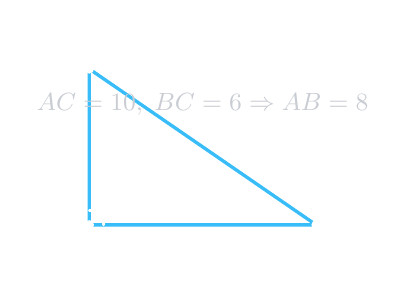
\begin{tikzpicture}[scale=0.9]
  \coordinate (A) at (0,2.2);
  \coordinate (B) at (0,0);
  \coordinate (C) at (3.2,0);
  \draw[new] (A)--(B)--(C)--cycle;
  \foreach \X/\pos in {A/above,B/below,C/below right}
    \node[dot,label={[lab]\pos:$\X$}] at (\X) {};
  \draw[base] ($(B)+(0.2,0)$) -- ($(B)+(0.2,0.2)$) -- ($(B)+(0,0.2)$);
  \node[labm] at (1.6,1.7) {$AC=10,\;BC=6 \Rightarrow AB=8$};
\end{tikzpicture}
\end{StepDiagram}

\Step{2} Given $x=30^\circ$ at $A$ means $\angle BAE=30^\circ$.
Since $AB$ is a diameter, $\angle AEB=90^\circ$, so
\[
\angle ABE=180^\circ-90^\circ-30^\circ=60^\circ.
\]

\begin{StepDiagram}
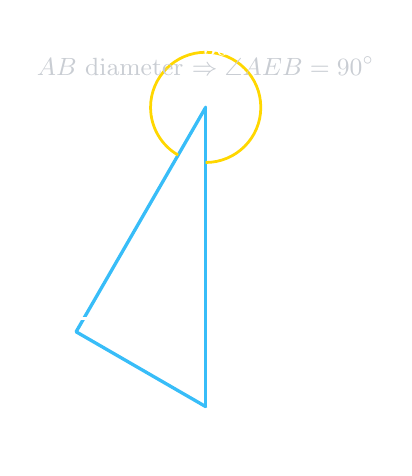
\begin{tikzpicture}[scale=0.95]
  \def\r{2.0}
  \coordinate (O) at (0,0);
  \coordinate (A) at (0,\r);
  \coordinate (B) at (0,-\r);
  \coordinate (E) at ({\r*cos(210)},{\r*sin(210)});
  \draw[base] (O) circle (\r);
  \foreach \X/\pos in {A/above,B/below,E/left}
    \node[dot,label={[lab]\pos:$\X$}] at (\X) {};
  \draw[new] (A)--(B);
  \draw[new] (A)--(E) (B)--(E);
  \draw[base] ($(E)+(0.18,0)$) -- ($(E)+(0.18,0.18)$) -- ($(E)+(0,0.18)$);
  \pic[ang,"$30^\circ$",lab,angle radius=7mm,angle eccentricity=1.15] {angle=B--A--E};
  \node[labm] at (0,2.55) {$AB$ diameter $\Rightarrow \angle AEB=90^\circ$};
\end{tikzpicture}
\end{StepDiagram}

\Step{3} Tangent--chord theorem:
\[
\angle EBD = \angle BAE = 30^\circ.
\]

\begin{StepDiagram}
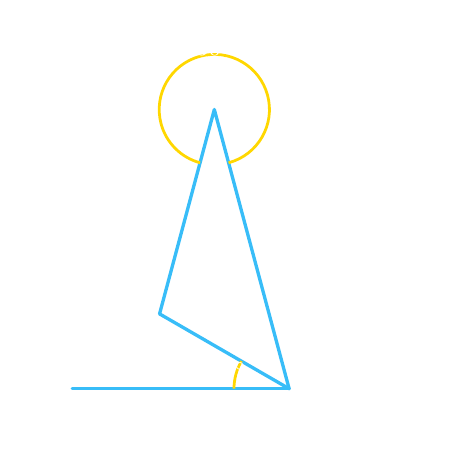
\begin{tikzpicture}[scale=0.95]
  \def\r{2.0}
  \coordinate (O) at (0,0);
  \coordinate (B) at (0,-\r);
  \coordinate (A) at ({\r*cos(120)},{\r*sin(120)});
  \coordinate (E) at ({\r*cos(210)},{\r*sin(210)});
  \coordinate (D) at (-2.9,-\r);
  \draw[base] (O) circle (\r);
  \foreach \X/\pos in {B/below,A/above left,E/left,D/below left}
    \node[dot,label={[lab]\pos:$\X$}] at (\X) {};
  \draw[new] (B)--(D); % tangent
  \draw[new] (B)--(E); % chord
  \draw[new] (A)--(B) (A)--(E);
  \pic[ang,"$30^\circ$",lab,angle radius=7mm,angle eccentricity=1.15] {angle=E--B--D};
  \pic[ang,"$30^\circ$",lab,angle radius=7mm,angle eccentricity=1.15] {angle=B--A--E};
\end{tikzpicture}
\end{StepDiagram}

\[
\boxed{r=4\text{ cm},\quad \angle ABE=60^\circ,\quad \angle ABC=90^\circ,\quad \angle EBD=30^\circ}
\]
\end{QAPair}

% ============================================================
% Q7
\begin{QAPair}{Question 7}
\textcolor{gold}{\bfseries Question:} In the figure, $ABCD$ is a square having side $10$ cm.
Triangle $BOP$ is enlarged as triangle $BCQ$. Find:
(i) scale factor of enlargement if $OP=2$ cm
(ii) $CQ$
(iii) $\angle BQC$ and $\angle BPO$
(iv) $AO$
(v) $AR$.
\tcblower
\textcolor{green}{\bfseries Answer:}\par

\Step{1} $BC=10$ cm and $O$ is midpoint of $BC$ (centre on diameter $BC$), so $BO=5$ cm.
Hence scale factor
\[
k=\frac{BC}{BO}=\frac{10}{5}=2.
\]

\begin{StepDiagram}
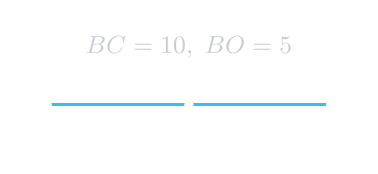
\begin{tikzpicture}[scale=0.9]
  \coordinate (B) at (0,0);
  \coordinate (C) at (4,0);
  \coordinate (O) at (2,0);
  \draw[new] (B)--(C);
  \node[dot,label={[lab]below:$B$}] at (B) {};
  \node[dot,label={[lab]below:$C$}] at (C) {};
  \node[dot,label={[lab]above:$O$}] at (O) {};
  \node[labm] at (2,0.8) {$BC=10,\;BO=5$};
\end{tikzpicture}
\end{StepDiagram}

\Step{2} $OP$ corresponds to $CQ$, so
\[
CQ=k\cdot OP=2\times 2=4\text{ cm}.
\]

\begin{StepDiagram}
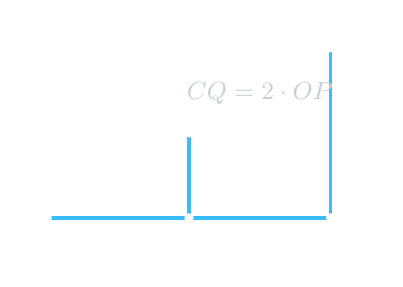
\begin{tikzpicture}[scale=0.9]
  \coordinate (B) at (0,0);
  \coordinate (O) at (2,0);
  \coordinate (C) at (4,0);
  \coordinate (P) at (2,1.2);
  \coordinate (Q) at (4,2.4);
  \draw[new] (B)--(C);
  \draw[new] (O)--(P);
  \draw[new] (C)--(Q);
  \foreach \X/\pos in {B/below,O/below,C/below,P/left,Q/right}
    \node[dot,label={[lab]\pos:$\X$}] at (\X) {};
  \node[labm] at (3,1.75) {$CQ=2\cdot OP$};
\end{tikzpicture}
\end{StepDiagram}

\Step{3} Since $BC$ is a diameter and $Q$ lies on the circle,
\[
\angle BQC=90^\circ.
\]
Enlargement preserves angles $\Rightarrow \angle BPO=90^\circ$.

\begin{StepDiagram}
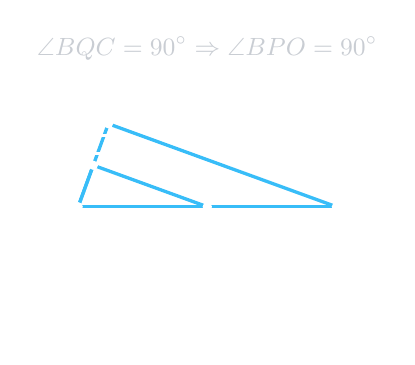
\begin{tikzpicture}[scale=0.82]
  % square reference (small)
  \coordinate (B) at (0,0);
  \coordinate (C) at (4,0);
  \coordinate (O) at (2,0);
  \def\r{2}
  \coordinate (Q) at ($(O)+(140:\r)$);
  \coordinate (P) at ($(B)!0.5!(Q)$); % schematic preimage
  \draw[base] (O) circle (\r);
  \draw[new] (B)--(C);
  \draw[new] (B)--(Q) (C)--(Q);
  \draw[new] (B)--(P) (O)--(P);
  \foreach \X/\pos in {B/below,C/below,O/below,Q/above,P/left}
    \node[dot,label={[lab]\pos:$\X$}] at (\X) {};
  \draw[base] ($(Q)+(-0.18,0)$) -- ($(Q)+(-0.18,-0.18)$) -- ($(Q)+(0,-0.18)$);
  \draw[base] ($(P)+(0.18,0)$) -- ($(P)+(0.18,0.18)$) -- ($(P)+(0,0.18)$);
  \node[labm] at (2,2.45) {$\angle BQC=90^\circ \Rightarrow \angle BPO=90^\circ$};
\end{tikzpicture}
\end{StepDiagram}

\Step{4} Using coordinates in the square, $AO=\sqrt{10^2+5^2}=5\sqrt5$ cm.

\begin{StepDiagram}
\begin{tikzpicture}[scale=0.65]
  \coordinate (A) at (0,0);
  \coordinate (B) at (4,0);
  \coordinate (C) at (4,4);
  \coordinate (D) at (0,4);
  \coordinate (O) at (4,2);
  \draw[base] (A)--(B)--(C)--(D)--cycle;
  \draw[new] (A)--(O);
  \foreach \X/\pos in {A/below left,B/below,C/above right,D/above left,O/right}
    \node[dot,label={[lab]\pos:$\X$}] at (\X) {};
  \node[labm] at (1.9,-0.65) {$AO=\sqrt{10^2+5^2}=5\sqrt5$ (scaled view)};
\end{tikzpicture}
\end{StepDiagram}

\Step{5} Radius is $5$ cm, so tangent point gives $BR=5$ and
\[
AR=AB+BR=10+5=15\text{ cm}.
\]

\begin{StepDiagram}
\begin{tikzpicture}[scale=0.7]
  \coordinate (A) at (0,0);
  \coordinate (B) at (4,0);
  \coordinate (C) at (4,4);
  \coordinate (O) at (4,2);
  \def\r{2}
  \coordinate (R) at (6,0);
  \draw[base] (A)--(B)--(C);
  \draw[base] (O) circle (\r);
  \draw[new] (B)--(R);
  \foreach \X/\pos in {A/below,B/below,C/above,O/right,R/below}
    \node[dot,label={[lab]\pos:$\X$}] at (\X) {};
  \node[labm] at (3.0,-0.8) {$BR=r=5 \Rightarrow AR=10+5=15$};
\end{tikzpicture}
\end{StepDiagram}

\[
\boxed{
\begin{aligned}
k&=2,\quad CQ=4\text{ cm},\quad \angle BQC=90^\circ,\\
\angle BPO&=90^\circ,\quad AO=5\sqrt5\text{ cm},\quad AR=15\text{ cm}.
\end{aligned}}
\]
\end{QAPair}

% ============================================================
% Q8
\begin{QAPair}{Question 8}
\textcolor{gold}{\bfseries Question:} In the adjoining figure, $\angle QPR=60^\circ$. Find:
(i) $\angle QSR$
(ii) $\angle PRS$
(iii) $\angle PQS$
(iv) $\angle QTR$
(v) Why $\angle QTR$ is an acute angle?
\tcblower
\textcolor{green}{\bfseries Answer:}\par

\Step{1} $\angle QPR$ and $\angle QSR$ subtend the same chord $QR$:
\[
\angle QSR=60^\circ.
\]

\begin{StepDiagram}
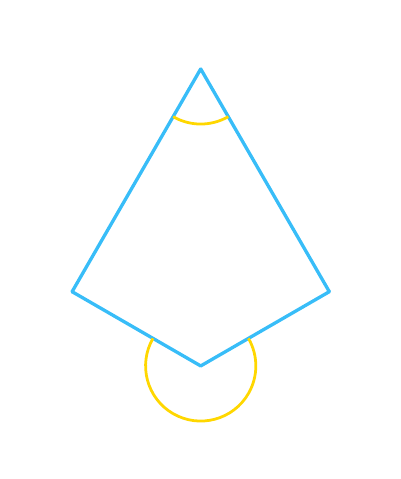
\begin{tikzpicture}[scale=0.92]
  \def\r{2.05}
  \coordinate (O) at (0,0);
  \coordinate (P) at (0,\r);
  \coordinate (S) at (0,-\r);
  \coordinate (Q) at ({\r*cos(210)},{\r*sin(210)});
  \coordinate (R) at ({\r*cos(330)},{\r*sin(330)});
  \draw[base] (O) circle (\r);
  \foreach \X/\pos in {P/above,S/below,Q/left,R/right}
    \node[dot,label={[lab]\pos:$\X$}] at (\X) {};
  \draw[new] (P)--(Q) (P)--(R);
  \draw[new] (S)--(Q) (S)--(R);
  \pic[ang,"$60^\circ$",lab,angle radius=7mm,angle eccentricity=1.2] {angle=Q--P--R};
  \pic[ang,"$60^\circ$",lab,angle radius=7mm,angle eccentricity=1.2] {angle=Q--S--R};
\end{tikzpicture}
\end{StepDiagram}

\Step{2} $PS$ is a diameter $\Rightarrow$ angles in a semicircle:
\[
\angle PRS=90^\circ,\qquad \angle PQS=90^\circ.
\]

\begin{StepDiagram}
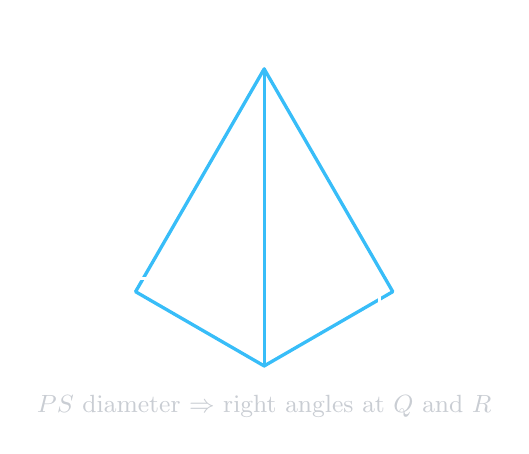
\begin{tikzpicture}[scale=0.92]
  \def\r{2.05}
  \coordinate (O) at (0,0);
  \coordinate (P) at (0,\r);
  \coordinate (S) at (0,-\r);
  \coordinate (Q) at ({\r*cos(210)},{\r*sin(210)});
  \coordinate (R) at ({\r*cos(330)},{\r*sin(330)});
  \draw[base] (O) circle (\r);
  \foreach \X/\pos in {P/above,S/below,Q/left,R/right}
    \node[dot,label={[lab]\pos:$\X$}] at (\X) {};
  \draw[new] (P)--(S);
  \draw[new] (R)--(P) (R)--(S);
  \draw[new] (Q)--(P) (Q)--(S);
  \draw[base] ($(R)+(-0.18,0)$) -- ($(R)+(-0.18,-0.18)$) -- ($(R)+(0,-0.18)$);
  \draw[base] ($(Q)+(0.18,0)$) -- ($(Q)+(0.18,0.18)$) -- ($(Q)+(0,0.18)$);
  \node[labm] at (0,-2.6) {$PS$ diameter $\Rightarrow$ right angles at $Q$ and $R$};
\end{tikzpicture}
\end{StepDiagram}

\Step{3} $\angle QTR$ also subtends chord $QR$, so
\[
\angle QTR=60^\circ.
\]

\begin{StepDiagram}
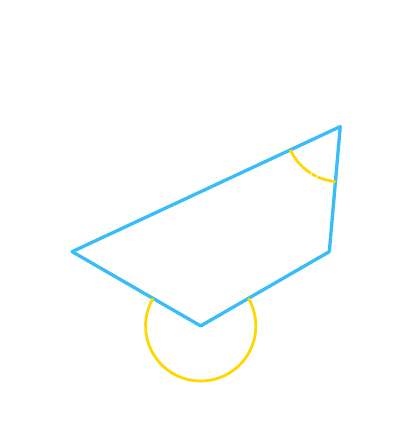
\begin{tikzpicture}[scale=0.92]
  \def\r{2.05}
  \coordinate (O) at (0,0);
  \coordinate (Q) at ({\r*cos(210)},{\r*sin(210)});
  \coordinate (R) at ({\r*cos(330)},{\r*sin(330)});
  \coordinate (T) at ({\r*cos(20)},{\r*sin(20)});
  \coordinate (S) at (0,-\r);
  \draw[base] (O) circle (\r);
  \foreach \X/\pos in {Q/left,R/right,T/above right,S/below}
    \node[dot,label={[lab]\pos:$\X$}] at (\X) {};
  \draw[new] (T)--(Q) (T)--(R);
  \draw[new] (S)--(Q) (S)--(R);
  \pic[ang,"$60^\circ$",lab,angle radius=7mm,angle eccentricity=1.2] {angle=Q--T--R};
  \pic[ang,"$60^\circ$",lab,angle radius=7mm,angle eccentricity=1.2] {angle=Q--S--R};
\end{tikzpicture}
\end{StepDiagram}

\Step{4} $\angle QTR$ is half the \emph{minor} arc $QR$ and minor arc $QR<180^\circ$,
so $\angle QTR<90^\circ$ (acute).

\EqDiagram{\text{minor arc }QR<180^\circ \;\Rightarrow\; \angle QTR=\tfrac12(\text{minor arc }QR)<90^\circ.}

\[
\boxed{\angle QSR=60^\circ,\;\angle PRS=90^\circ,\;\angle PQS=90^\circ,\;\angle QTR=60^\circ}
\]
\end{QAPair}

% ============================================================
% Q9
\begin{QAPair}{Question 9}
\textcolor{gold}{\bfseries Question:} In the figure, $P$ is the centre of the circle and $\angle BPD=130^\circ$.
Find:
(i) $\angle BAD$
(ii) $\angle BCD$
(iii) $\angle ABC+\angle ADC$.
\tcblower
\textcolor{green}{\bfseries Answer:}\par

\Step{1} Inscribed angle on the same arc is half the central angle:
\[
\angle BAD=\frac12\cdot 130^\circ=65^\circ.
\]

\begin{StepDiagram}
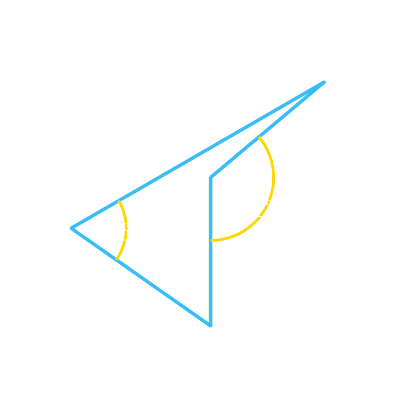
\begin{tikzpicture}[scale=0.92]
  \def\r{2.05}
  \coordinate (P) at (0,0);
  \coordinate (B) at (0,-\r);
  \coordinate (D) at ({\r*cos(40)},{\r*sin(40)});
  \coordinate (A) at ({\r*cos(200)},{\r*sin(200)});
  \draw[base] (P) circle (\r);
  \foreach \X/\pos in {P/right,B/below,D/above right,A/left}
    \node[dot,label={[lab]\pos:$\X$}] at (\X) {};
  \draw[new] (P)--(B) (P)--(D);
  \draw[new] (A)--(B) (A)--(D);
  \pic[ang,"$130^\circ$",lab,angle radius=8mm,angle eccentricity=1.15] {angle=B--P--D};
  \pic[ang,"$65^\circ$",lab,angle radius=7mm,angle eccentricity=1.2] {angle=B--A--D};
\end{tikzpicture}
\end{StepDiagram}

\Step{2} If $C$ lies on the minor arc $BD$, then $\angle BCD$ subtends the major arc:
\[
\text{major arc }BD=360^\circ-130^\circ=230^\circ\Rightarrow \angle BCD=115^\circ.
\]

\begin{StepDiagram}
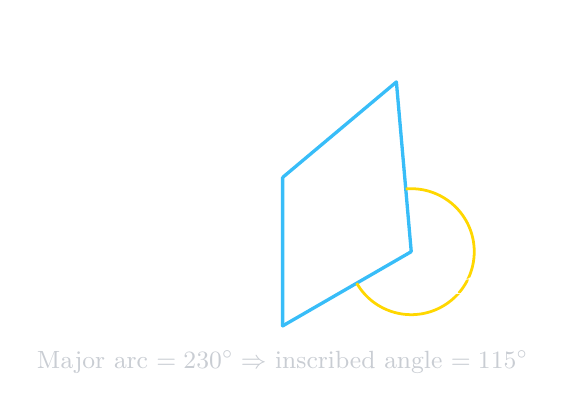
\begin{tikzpicture}[scale=0.92]
  \def\r{2.05}
  \coordinate (P) at (0,0);
  \coordinate (B) at (0,-\r);
  \coordinate (D) at ({\r*cos(40)},{\r*sin(40)});
  \coordinate (C) at ({\r*cos(330)},{\r*sin(330)});
  \draw[base] (P) circle (\r);
  \foreach \X/\pos in {P/right,B/below,D/above right,C/right}
    \node[dot,label={[lab]\pos:$\X$}] at (\X) {};
  \draw[new] (C)--(B) (C)--(D);
  \draw[new] (P)--(B) (P)--(D);
  \pic[ang,"$115^\circ$",lab,angle radius=8mm,angle eccentricity=1.15] {angle=B--C--D};
  \node[labm] at (0,-2.55) {Major arc $=230^\circ \Rightarrow$ inscribed angle $=115^\circ$};
\end{tikzpicture}
\end{StepDiagram}

\Step{3} In cyclic quadrilateral $ABCD$, opposite angles are supplementary:
\[
\angle ABC+\angle ADC=180^\circ.
\]

\EqDiagram{\angle ABC+\angle ADC=180^\circ \quad (\text{opposite angles in a cyclic quadrilateral}).}

\[
\boxed{\angle BAD=65^\circ,\quad \angle BCD=115^\circ,\quad \angle ABC+\angle ADC=180^\circ}
\]
\end{QAPair}

% ============================================================
% Q10
\begin{QAPair}{Question 10}
\textcolor{gold}{\bfseries Question:} In the given figure, $PQ\parallel SR$ and $\angle QPS=95^\circ$. Find:
(i) $\angle QRS$
(ii) $\angle PQR$
(iii) $\angle PSR$.
\tcblower
\textcolor{green}{\bfseries Answer:}\par

\Step{1} Since $PQ\parallel SR$ with transversal $PS$:
\[
\angle PSR=\angle QPS=95^\circ.
\]

\begin{StepDiagram}
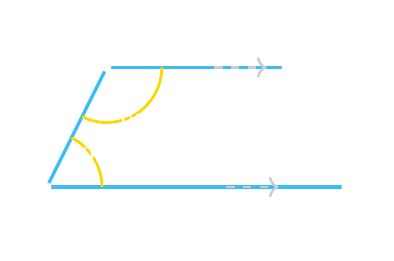
\begin{tikzpicture}[scale=0.95]
  \coordinate (P) at (-2,0);
  \coordinate (Q) at (2,0);
  \coordinate (S) at (-1.2,1.6);
  \coordinate (R) at (1.2,1.6);
  \draw[new] (P)--(Q);
  \draw[new] (S)--(R);
  \draw[new] (P)--(S);
  \draw[help,->] ($(P)!0.6!(Q)$) -- ($(P)!0.6!(Q)+(0.7,0)$);
  \draw[help,->] ($(S)!0.6!(R)$) -- ($(S)!0.6!(R)+(0.7,0)$);
  \foreach \X/\pos in {P/below,Q/below,S/above left,R/above right}
    \node[dot,label={[lab]\pos:$\X$}] at (\X) {};
  \pic[ang,"$95^\circ$",lab,angle radius=7mm,angle eccentricity=1.15] {angle=Q--P--S};
  \pic[ang,"$95^\circ$",lab,angle radius=7mm,angle eccentricity=1.15] {angle=P--S--R};
\end{tikzpicture}
\end{StepDiagram}

\Step{2} In cyclic quadrilateral, opposite angles are supplementary:
\[
\angle QRS=180^\circ-95^\circ=85^\circ.
\]

\EqDiagram{\angle QRS+\angle QPS=180^\circ \Rightarrow \angle QRS=85^\circ.}

\Step{3} Angles subtending the same chord $PR$ are equal:
\[
\angle PQR=\angle PSR=95^\circ.
\]

\begin{StepDiagram}
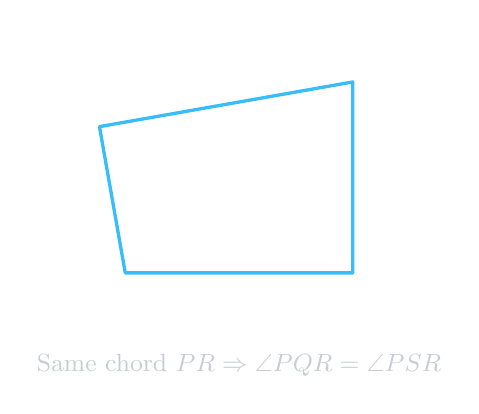
\begin{tikzpicture}[scale=0.92]
  \def\r{2.05}
  \coordinate (O) at (0,0);
  \coordinate (P) at ({\r*cos(220)},{\r*sin(220)});
  \coordinate (Q) at ({\r*cos(320)},{\r*sin(320)});
  \coordinate (R) at ({\r*cos(40)},{\r*sin(40)});
  \coordinate (S) at ({\r*cos(160)},{\r*sin(160)});
  \draw[base] (O) circle (\r);
  \foreach \X/\pos in {P/below left,Q/below right,R/above right,S/above left}
    \node[dot,label={[lab]\pos:$\X$}] at (\X) {};
  \draw[new] (P)--(Q)--(R)--(S)--cycle;
  \node[labm] at (0,-2.6) {Same chord $PR \Rightarrow \angle PQR=\angle PSR$};
\end{tikzpicture}
\end{StepDiagram}

\[
\boxed{\angle QRS=85^\circ,\quad \angle PQR=95^\circ,\quad \angle PSR=95^\circ}
\]
\end{QAPair}

% ============================================================
% Q11
\begin{QAPair}{Question 11}
\textcolor{gold}{\bfseries Question:} In the adjoining figure, $\angle ADC=120^\circ$.
(i) Find $\angle BAC$.
(ii) Find $\angle CAD$ if $AD=CD$.
\tcblower
\textcolor{green}{\bfseries Answer:}\par

\Step{1} $\angle ADC=120^\circ$ subtends arc $AC$ (not containing $D$), so that arc is $240^\circ$.
Hence minor arc $AC$ is $120^\circ$.

\EqDiagram{\text{arc }AC=2\angle ADC=240^\circ \Rightarrow \text{minor arc }AC=120^\circ.}

\Step{2} With $AB$ a diameter, arc $AB=180^\circ$.
Arc $AC$ through $B$ is $240^\circ$, so arc $BC=60^\circ$.
Thus
\[
\angle BAC=\frac12(60^\circ)=30^\circ.
\]

\begin{StepDiagram}
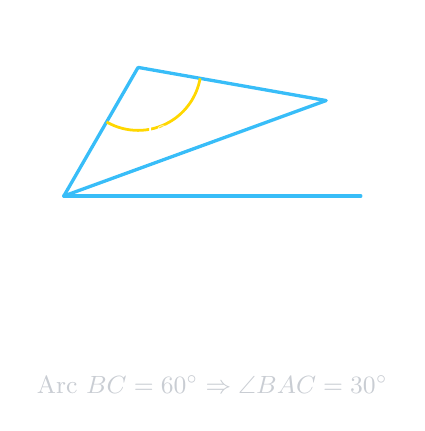
\begin{tikzpicture}[scale=0.92]
  \def\r{2.05}
  \coordinate (P) at (0,0);
  \coordinate (A) at (-\r,0);
  \coordinate (B) at (\r,0);
  \coordinate (D) at ({\r*cos(120)},{\r*sin(120)});
  \coordinate (C) at ({\r*cos(40)},{\r*sin(40)});
  \draw[base] (P) circle (\r);
  \foreach \X/\pos in {A/below,B/below,C/above right,D/above left}
    \node[dot,label={[lab]\pos:$\X$}] at (\X) {};
  \draw[new] (A)--(B); % diameter
  \draw[new] (A)--(C);
  \draw[new] (D)--(A) (D)--(C);
  \pic[ang,"$120^\circ$",lab,angle radius=8mm,angle eccentricity=1.15] {angle=A--D--C};
  \node[labm] at (0,-2.6) {Arc $BC=60^\circ \Rightarrow \angle BAC=30^\circ$};
\end{tikzpicture}
\end{StepDiagram}

\Step{3} If $AD=CD$, then $\triangle ACD$ is isosceles:
\[
2\angle CAD + 120^\circ = 180^\circ \Rightarrow \angle CAD=30^\circ.
\]

\begin{StepDiagram}
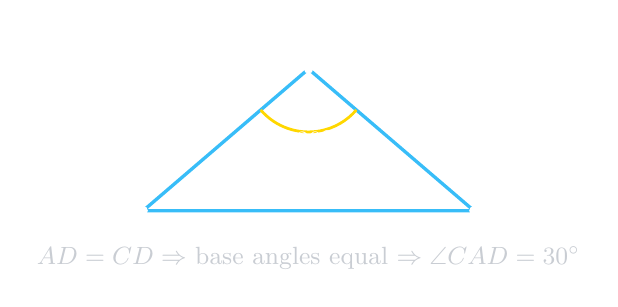
\begin{tikzpicture}[scale=1.0]
  \coordinate (A) at (-2.1,0);
  \coordinate (C) at (2.1,0);
  \coordinate (D) at (0,1.8);
  \draw[new] (A)--(D)--(C)--cycle;
  \foreach \X/\pos in {A/below,C/below,D/above}
    \node[dot,label={[lab]\pos:$\X$}] at (\X) {};
  \pic[ang,"$120^\circ$",lab,angle radius=8mm,angle eccentricity=1.12] {angle=A--D--C};
  \node[labm] at (0,-0.6) {$AD=CD \Rightarrow$ base angles equal $\Rightarrow \angle CAD=30^\circ$};
\end{tikzpicture}
\end{StepDiagram}

\[
\boxed{\angle BAC=30^\circ \qquad \angle CAD=30^\circ}
\]
\end{QAPair}

% ============================================================
% Q12
\begin{QAPair}{Question 12}
\textcolor{gold}{\bfseries Question:} In the figure, $\angle ABE=95^\circ$ and $\angle BAE=65^\circ$.
Find (i) $\angle ECD$ (ii) $\angle CDE$ (iii) $\angle CED$.
\tcblower
\textcolor{green}{\bfseries Answer:}\par

\Step{1} $E$ lies on extension of $BC$, so $\angle ABE$ is exterior:
\[
\angle ABC = 180^\circ-95^\circ=85^\circ.
\]

\begin{StepDiagram}
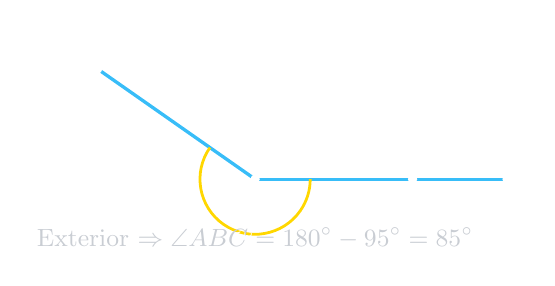
\begin{tikzpicture}[scale=1.0]
  \coordinate (B) at (0,0);
  \coordinate (A) at (-2,1.4);
  \coordinate (C) at (2,0);
  \coordinate (E) at (3.2,0);
  \draw[new] (B)--(A);
  \draw[new] (B)--(C)--(E);
  \foreach \X/\pos in {A/above,B/below,C/below,E/below}
    \node[dot,label={[lab]\pos:$\X$}] at (\X) {};
  \pic[ang,"$95^\circ$",lab,angle radius=7mm,angle eccentricity=1.15] {angle=A--B--E};
  \node[labm] at (0,-0.75) {Exterior $\Rightarrow \angle ABC=180^\circ-95^\circ=85^\circ$};
\end{tikzpicture}
\end{StepDiagram}

\Step{2} $D$ lies on extension of $AE$, so $\angle BAE=\angle BAD=65^\circ$.
In cyclic quadrilateral $ABCD$:
\[
\angle BCD=180^\circ-65^\circ=115^\circ \Rightarrow \angle ECD=180^\circ-115^\circ=65^\circ.
\]

\begin{StepDiagram}
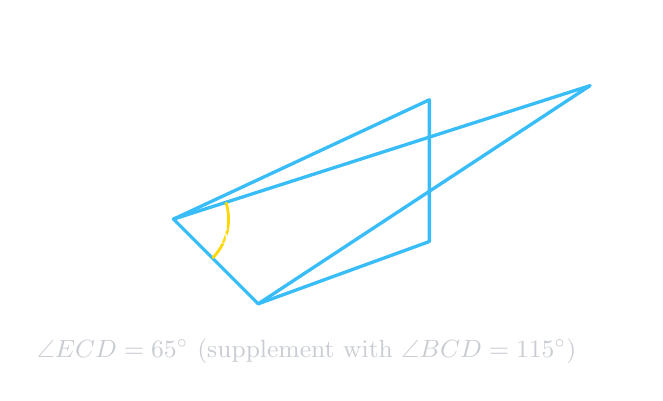
\begin{tikzpicture}[scale=0.9]
  \def\r{2.0}
  \coordinate (O) at (0,0);
  \coordinate (A) at ({\r*cos(200)},{\r*sin(200)});
  \coordinate (B) at ({\r*cos(250)},{\r*sin(250)});
  \coordinate (C) at ({\r*cos(330)},{\r*sin(330)});
  \coordinate (D) at ({\r*cos(30)},{\r*sin(30)});
  \coordinate (E) at (4.0,1.2);
  \draw[base] (O) circle (\r);
  \foreach \X/\pos in {A/left,B/below,C/below right,D/above right}
    \node[dot,label={[lab]\pos:$\X$}] at (\X) {};
  \node[dot,label={[lab]right:$E$}] at (E) {};
  \draw[new] (A)--(B)--(C)--(D)--cycle;
  \draw[new] (A)--(E) (B)--(E);
  \pic[ang,"$65^\circ$",lab,angle radius=7mm,angle eccentricity=1.15] {angle=B--A--E};
  \node[labm] at (0,-2.55) {$\angle ECD=65^\circ$ (supplement with $\angle BCD=115^\circ$)};
\end{tikzpicture}
\end{StepDiagram}

\Step{3} Opposite angles in cyclic quadrilateral:
\[
\angle ADC = 180^\circ-\angle ABC = 95^\circ.
\]
Since $DE$ is extension of $DA$:
\[
\angle CDE = 180^\circ-95^\circ=85^\circ.
\]

\begin{StepDiagram}
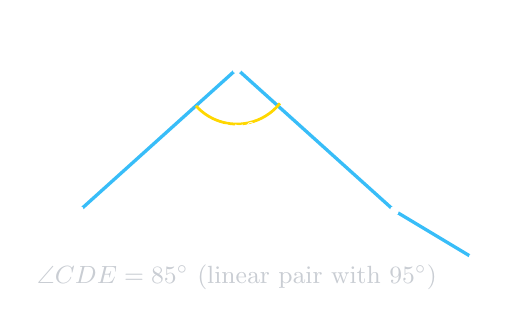
\begin{tikzpicture}[scale=1.0]
  \coordinate (D) at (0,1.8);
  \coordinate (C) at (-2,0);
  \coordinate (A) at (2,0);
  \coordinate (E) at (3.0,-0.6);
  \draw[new] (D)--(C);
  \draw[new] (D)--(A)--(E);
  \foreach \X/\pos in {D/above,C/below left,A/below,E/below}
    \node[dot,label={[lab]\pos:$\X$}] at (\X) {};
  \pic[ang,"$85^\circ$",lab,angle radius=7mm,angle eccentricity=1.15] {angle=C--D--E};
  \node[labm] at (0,-0.85) {$\angle CDE=85^\circ$ (linear pair with $95^\circ$)};
\end{tikzpicture}
\end{StepDiagram}

\Step{4} In $\triangle CDE$:
\[
\angle CED=180^\circ-65^\circ-85^\circ=30^\circ.
\]

\EqDiagram{\angle CED=180^\circ-\angle ECD-\angle CDE=180^\circ-65^\circ-85^\circ=30^\circ.}

\[
\boxed{\angle ECD=65^\circ,\quad \angle CDE=85^\circ,\quad \angle CED=30^\circ}
\]
\end{QAPair}

% ============================================================
% Q13
\begin{QAPair}{Question 13}
\textcolor{gold}{\bfseries Question:} A circular wall clock of radius $1$ ft is hung by a $4$ feet long string with a nail at $P$.
(i) Find distance between centre of clock and nail.
(ii) How far above the clock is the nail?
\tcblower
\textcolor{green}{\bfseries Answer:}\par

\Step{1} The string forms two equal tangents $PA$ and $PB$:
\[
PA=PB,\quad PA+PB=4 \Rightarrow PA=PB=2\text{ ft}.
\]

\begin{StepDiagram}
\begin{tikzpicture}[scale=0.92]
  \def\r{2.0}
  \coordinate (O) at (0,0);
  \coordinate (P) at (0,3.1);
  \coordinate (A) at ({\r*cos(140)},{\r*sin(140)});
  \coordinate (B) at ({\r*cos(40)},{\r*sin(40)});
  \draw[base] (O) circle (\r);
  \foreach \X/\pos in {O/below,P/above,A/left,B/right}
    \node[dot,label={[lab]\pos:$\X$}] at (\X) {};
  \draw[new] (P)--(A);
  \draw[new] (P)--(B);
  \node[labm] at (0,-2.55) {$PA=PB=2$ ft (equal tangents)};
\end{tikzpicture}
\end{StepDiagram}

\Step{2} In right $\triangle OAP$ (radius $\perp$ tangent), $OA=1$ and $PA=2$:
\[
OP=\sqrt{1^2+2^2}=\sqrt5\text{ ft}.
\]

\begin{StepDiagram}
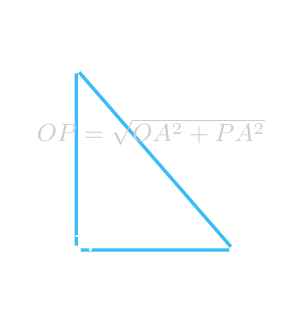
\begin{tikzpicture}[scale=1.0]
  \coordinate (O) at (0,0);
  \coordinate (A) at (-2,0);
  \coordinate (P) at (-2,2.3);
  \draw[new] (O)--(A)--(P)--cycle;
  \foreach \X/\pos in {O/right,A/below,P/above}
    \node[dot,label={[lab]\pos:$\X$}] at (\X) {};
  \draw[base] ($(A)+(0.18,0)$) -- ($(A)+(0.18,0.18)$) -- ($(A)+(0,0.18)$);
  \node[labm] at (-1.05,1.5) {$OP=\sqrt{OA^2+PA^2}$};
\end{tikzpicture}
\end{StepDiagram}

\Step{3} Nail height above the top of the clock:
\[
OP-r=\sqrt5-1\text{ ft}.
\]

\EqDiagram{\text{Height above clock}=OP-r=\sqrt5-1\text{ ft}.}

\[
\boxed{
\begin{aligned}
OP&=\sqrt5\text{ ft},\\
\text{height above clock}&=\sqrt5-1\text{ ft}.
\end{aligned}}
\]
\end{QAPair}

% ============================================================
% Q14
\begin{QAPair}{Question 14}
\textcolor{gold}{\bfseries Question:} A wooden wheel moving on the ground is $99$ cm away from a point $A$.
Find diameter of the wheel if the distance between centre of wheel and point $A$ is $101$ cm.
How much distance does the wheel cover in one round?
\tcblower
\textcolor{green}{\bfseries Answer:}\par

\Step{1} Right triangle $OBA$:
\[
101^2=r^2+99^2 \Rightarrow r^2=101^2-99^2=400 \Rightarrow r=20\text{ cm}.
\]
So diameter $d=40$ cm.

\begin{StepDiagram}
\begin{tikzpicture}[scale=0.95]
  \coordinate (B) at (0,0);
  \coordinate (A) at (4.2,0);
  \coordinate (O) at (0,2.0);
  \draw[base] (0,-0.1)--(4.8,-0.1);
  \draw[base] (O) circle (2.0);
  \draw[new] (O)--(A);
  \draw[new] (O)--(B);
  \draw[new] (B)--(A);
  \foreach \X/\pos in {B/below,A/below,O/right}
    \node[dot,label={[lab]\pos:$\X$}] at (\X) {};
  \draw[base] ($(B)+(0.18,0)$) -- ($(B)+(0.18,0.18)$) -- ($(B)+(0,0.18)$);
  \node[labm] at (2.0,1.3) {$OA=101,\;BA=99$};
\end{tikzpicture}
\end{StepDiagram}

\Step{2} Distance in one complete round is circumference:
\[
\text{distance}= \pi d = 40\pi\text{ cm}.
\]

\begin{StepDiagram}
\begin{tikzpicture}[scale=0.95]
  \coordinate (O) at (0,0);
  \draw[base] (O) circle (2.0);
  \node[dot,label={[lab]right:$O$}] at (O) {};
  \node[labm] at (0,-2.6) {One round = circumference $=\pi d$};
\end{tikzpicture}
\end{StepDiagram}

\[
\boxed{
\begin{aligned}
d&=40\text{ cm},\\
\text{distance in one round}&=40\pi\text{ cm}.
\end{aligned}}
\]
\end{QAPair}

\end{document}
